\documentclass{standalone}
\usepackage{tikz}
\usetikzlibrary{patterns, positioning}

\begin{document}
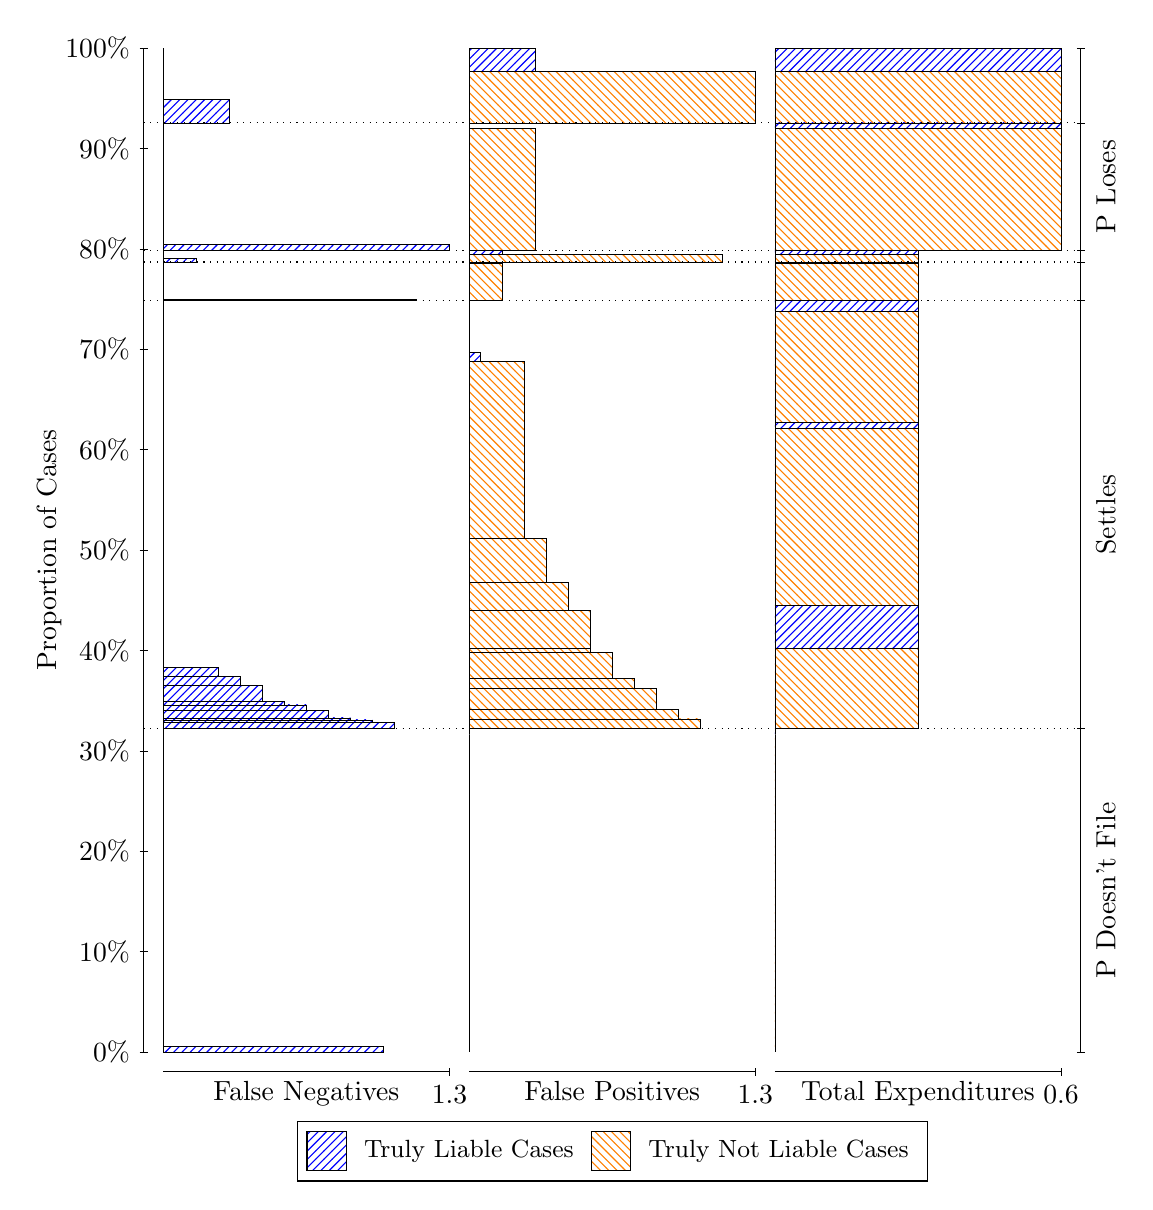
\begin{tikzpicture}
\draw[black, very thin] (1.5,1.75) -- (1.5,14.5);
\node[rotate=90, anchor=center] at (0.3, 8.125) {Proportion of Cases};
\draw[black, very thin] (1.45,1.75) -- (1.55,1.75);
\node[anchor=east] at (1.45, 1.75) {0\%};
\draw[black, very thin] (1.45,3.025) -- (1.55,3.025);
\node[anchor=east] at (1.45, 3.025) {10\%};
\draw[black, very thin] (1.45,4.3) -- (1.55,4.3);
\node[anchor=east] at (1.45, 4.3) {20\%};
\draw[black, very thin] (1.45,5.575) -- (1.55,5.575);
\node[anchor=east] at (1.45, 5.575) {30\%};
\draw[black, very thin] (1.45,6.85) -- (1.55,6.85);
\node[anchor=east] at (1.45, 6.85) {40\%};
\draw[black, very thin] (1.45,8.125) -- (1.55,8.125);
\node[anchor=east] at (1.45, 8.125) {50\%};
\draw[black, very thin] (1.45,9.4) -- (1.55,9.4);
\node[anchor=east] at (1.45, 9.4) {60\%};
\draw[black, very thin] (1.45,10.675) -- (1.55,10.675);
\node[anchor=east] at (1.45, 10.675) {70\%};
\draw[black, very thin] (1.45,11.95) -- (1.55,11.95);
\node[anchor=east] at (1.45, 11.95) {80\%};
\draw[black, very thin] (1.45,13.225) -- (1.55,13.225);
\node[anchor=east] at (1.45, 13.225) {90\%};
\draw[black, very thin] (1.45,14.5) -- (1.55,14.5);
\node[anchor=east] at (1.45, 14.5) {100\%};

\draw[black, very thin] (13.4,1.75) -- (13.4,14.5);
\draw[black, very thin] (13.35,1.75) -- (13.45,1.75);
\node[anchor=west] at (13.35, 1.75) {};
\draw[black, very thin] (13.35,5.856) -- (13.45,5.856);
\node[anchor=west] at (13.35, 5.856) {};
\draw[black, very thin] (13.35,11.295) -- (13.45,11.295);
\node[anchor=west] at (13.35, 11.295) {};
\draw[black, very thin] (13.35,11.782) -- (13.45,11.782);
\node[anchor=west] at (13.35, 11.782) {};
\draw[black, very thin] (13.35,11.933) -- (13.45,11.933);
\node[anchor=west] at (13.35, 11.933) {};
\draw[black, very thin] (13.35,13.55) -- (13.45,13.55);
\node[anchor=west] at (13.35, 13.55) {};
\draw[black, very thin] (13.35,14.5) -- (13.45,14.5);
\node[anchor=west] at (13.35, 14.5) {};

\draw[black, very thin, pattern color=blue, pattern=north east lines] (1.75,1.75) rectangle (4.5449,1.8217);
\draw[black, very thin, pattern color=orange, pattern=north west lines] (1.75,1.8217) rectangle (1.75,5.856);
\draw[black, very thin, pattern color=blue, pattern=north east lines] (1.75,5.856) rectangle (4.6846,5.9385);
\draw[black, very thin, pattern color=blue, pattern=north east lines] (1.75,5.9385) rectangle (4.4051,5.9686);
\draw[black, very thin, pattern color=blue, pattern=north east lines] (1.75,5.9686) rectangle (4.1256,5.9934);
\draw[black, very thin, pattern color=blue, pattern=north east lines] (1.75,5.9934) rectangle (3.8462,6.0865);
\draw[black, very thin, pattern color=blue, pattern=north east lines] (1.75,6.0865) rectangle (3.5667,6.159);
\draw[black, very thin, pattern color=blue, pattern=north east lines] (1.75,6.159) rectangle (3.2872,6.2008);
\draw[black, very thin, pattern color=blue, pattern=north east lines] (1.75,6.2008) rectangle (3.0077,6.4016);
\draw[black, very thin, pattern color=blue, pattern=north east lines] (1.75,6.4016) rectangle (2.7282,6.5181);
\draw[black, very thin, pattern color=blue, pattern=north east lines] (1.75,6.5181) rectangle (2.4487,6.6314);
\draw[black, very thin, pattern color=orange, pattern=north west lines] (1.75,6.6314) rectangle (1.75,11.295);
\draw[black, very thin, pattern color=blue, pattern=north east lines] (1.75,11.295) rectangle (4.9641,11.305);
\draw[black, very thin, pattern color=orange, pattern=north west lines] (1.75,11.305) rectangle (1.75,11.782);
\draw[black, very thin, pattern color=blue, pattern=north east lines] (1.75,11.782) rectangle (2.1692,11.833);
\draw[black, very thin, pattern color=orange, pattern=north west lines] (1.75,11.833) rectangle (1.75,11.933);
\draw[black, very thin, pattern color=blue, pattern=north east lines] (1.75,11.933) rectangle (5.3833,12.005);
\draw[black, very thin, pattern color=orange, pattern=north west lines] (1.75,12.005) rectangle (1.75,13.55);
\draw[black, very thin, pattern color=blue, pattern=north east lines] (1.75,13.55) rectangle (2.5885,13.845);
\draw[black, very thin, pattern color=orange, pattern=north west lines] (1.75,13.845) rectangle (1.75,14.5);
\draw[black, very thin, pattern color=orange, pattern=north west lines] (5.6333,1.75) rectangle (5.6333,5.7843);
\draw[black, very thin, pattern color=blue, pattern=north east lines] (5.6333,5.7843) rectangle (5.6333,5.856);
\draw[black, very thin, pattern color=orange, pattern=north west lines] (5.6333,5.856) rectangle (8.5679,5.9793);
\draw[black, very thin, pattern color=orange, pattern=north west lines] (5.6333,5.9793) rectangle (8.2885,6.0984);
\draw[black, very thin, pattern color=orange, pattern=north west lines] (5.6333,6.0984) rectangle (8.009,6.3719);
\draw[black, very thin, pattern color=orange, pattern=north west lines] (5.6333,6.3719) rectangle (7.7295,6.4935);
\draw[black, very thin, pattern color=orange, pattern=north west lines] (5.6333,6.4935) rectangle (7.45,6.8221);
\draw[black, very thin, pattern color=orange, pattern=north west lines] (5.6333,6.8221) rectangle (7.1705,6.8716);
\draw[black, very thin, pattern color=orange, pattern=north west lines] (5.6333,6.8716) rectangle (7.1705,7.3539);
\draw[black, very thin, pattern color=orange, pattern=north west lines] (5.6333,7.3539) rectangle (6.891,7.7107);
\draw[black, very thin, pattern color=orange, pattern=north west lines] (5.6333,7.7107) rectangle (6.6115,8.2733);
\draw[black, very thin, pattern color=orange, pattern=north west lines] (5.6333,8.2733) rectangle (6.3321,10.519);
\draw[black, very thin, pattern color=blue, pattern=north east lines] (5.6333,10.519) rectangle (5.7731,10.633);
\draw[black, very thin, pattern color=blue, pattern=north east lines] (5.6333,10.633) rectangle (5.6333,11.295);
\draw[black, very thin, pattern color=orange, pattern=north west lines] (5.6333,11.295) rectangle (6.0526,11.771);
\draw[black, very thin, pattern color=blue, pattern=north east lines] (5.6333,11.771) rectangle (5.6333,11.782);
\draw[black, very thin, pattern color=orange, pattern=north west lines] (5.6333,11.782) rectangle (8.8474,11.882);
\draw[black, very thin, pattern color=blue, pattern=north east lines] (5.6333,11.882) rectangle (6.0526,11.933);
\draw[black, very thin, pattern color=orange, pattern=north west lines] (5.6333,11.933) rectangle (6.4718,13.478);
\draw[black, very thin, pattern color=blue, pattern=north east lines] (5.6333,13.478) rectangle (5.6333,13.55);
\draw[black, very thin, pattern color=orange, pattern=north west lines] (5.6333,13.55) rectangle (9.2667,14.206);
\draw[black, very thin, pattern color=blue, pattern=north east lines] (5.6333,14.206) rectangle (6.4718,14.5);
\draw[black, very thin, pattern color=orange, pattern=north west lines] (9.5167,1.75) rectangle (9.5167,5.7843);
\draw[black, very thin, pattern color=blue, pattern=north east lines] (9.5167,5.7843) rectangle (9.5167,5.856);
\draw[black, very thin, pattern color=orange, pattern=north west lines] (9.5167,5.856) rectangle (11.333,6.8716);
\draw[black, very thin, pattern color=blue, pattern=north east lines] (9.5167,6.8716) rectangle (11.333,7.4207);
\draw[black, very thin, pattern color=orange, pattern=north west lines] (9.5167,7.4207) rectangle (11.333,9.6667);
\draw[black, very thin, pattern color=blue, pattern=north east lines] (9.5167,9.6667) rectangle (11.333,9.7492);
\draw[black, very thin, pattern color=orange, pattern=north west lines] (9.5167,9.7492) rectangle (11.333,11.151);
\draw[black, very thin, pattern color=blue, pattern=north east lines] (9.5167,11.151) rectangle (11.333,11.295);
\draw[black, very thin, pattern color=orange, pattern=north west lines] (9.5167,11.295) rectangle (11.333,11.771);
\draw[black, very thin, pattern color=blue, pattern=north east lines] (9.5167,11.771) rectangle (11.333,11.782);
\draw[black, very thin, pattern color=orange, pattern=north west lines] (9.5167,11.782) rectangle (11.333,11.882);
\draw[black, very thin, pattern color=blue, pattern=north east lines] (9.5167,11.882) rectangle (11.333,11.933);
\draw[black, very thin, pattern color=orange, pattern=north west lines] (9.5167,11.933) rectangle (13.15,13.478);
\draw[black, very thin, pattern color=blue, pattern=north east lines] (9.5167,13.478) rectangle (13.15,13.55);
\draw[black, very thin, pattern color=orange, pattern=north west lines] (9.5167,13.55) rectangle (13.15,14.206);
\draw[black, very thin, pattern color=blue, pattern=north east lines] (9.5167,14.206) rectangle (13.15,14.5);
\draw[black, dotted] (1.5,5.856) -- (13.4,5.856);
\draw[black, dotted] (1.5,11.295) -- (13.4,11.295);
\draw[black, dotted] (1.5,11.782) -- (13.4,11.782);
\draw[black, dotted] (1.5,11.933) -- (13.4,11.933);
\draw[black, dotted] (1.5,13.55) -- (13.4,13.55);
\draw[black, very thin] (1.75,1.5) -- (5.3833,1.5);
\node[anchor=north] at (3.5667, 1.5) {False Negatives};
\draw[black, very thin] (5.3833,1.45) -- (5.3833,1.55);
\node[anchor=north] at (5.3833, 1.45) {1.3};

\draw[black, very thin] (5.6333,1.5) -- (9.2667,1.5);
\node[anchor=north] at (7.45, 1.5) {False Positives};
\draw[black, very thin] (9.2667,1.45) -- (9.2667,1.55);
\node[anchor=north] at (9.2667, 1.45) {1.3};

\draw[black, very thin] (9.5167,1.5) -- (13.15,1.5);
\node[anchor=north] at (11.333, 1.5) {Total Expenditures};
\draw[black, very thin] (13.15,1.45) -- (13.15,1.55);
\node[anchor=north] at (13.15, 1.45) {0.6};

\node[black, centered, rotate=90] at (13.72, 3.803) {P Doesn't File};
\node[black, centered, rotate=90] at (13.72, 8.5754) {Settles};


\node[black, centered, rotate=90] at (13.72, 12.741) {P Loses};


\draw (7.449999999999999,1.5) node[draw=none] (baseCoordinate) {};
\begin{scope}[align=center]
        \matrix[scale=0.5, draw=black, below=0.5cm of baseCoordinate, nodes={draw}, column sep=0.1cm]{
            \node[rectangle, draw, minimum width=0.5cm, minimum height=0.5cm, pattern=north east lines, pattern color=blue] {}; &
            \node[draw=none, font=\small] (B) {Truly Liable Cases}; &
            \node[rectangle, draw, minimum width=0.5cm, minimum height=0.5cm, pattern=north west lines, pattern color=orange] {}; &
            \node[draw=none, font=\small] (B) {Truly Not Liable Cases}; \\
            };
\end{scope}

\end{tikzpicture}
\end{document}